% This is LLNCS.DOC the documentation file of
% the LaTeX2e class from Springer-Verlag
% for Lecture Notes in Computer Science, version 2.4
\documentclass{llncs}
\usepackage{llncsdoc}
\usepackage{listings}
\usepackage{color}
\usepackage{graphicx}
\usepackage{pdfpages}
\definecolor{mygreen}{rgb}{0,0.6,0}
\definecolor{mygray}{rgb}{0.5,0.5,0.5}
\definecolor{mymauve}{rgb}{0.58,0,0.82}

\lstset{ %
  backgroundcolor=\color{white},   % choose the background color; you must add \usepackage{color} or \usepackage{xcolor}
  basicstyle=\footnotesize,        % the size of the fonts that are used for the code
  breakatwhitespace=false,         % sets if automatic breaks should only happen at whitespace
  breaklines=true,                 % sets automatic line breaking
  captionpos=b,                    % sets the caption-position to bottom
  commentstyle=\color{mygreen},    % comment style
  deletekeywords={...},            % if you want to delete keywords from the given language
  escapeinside={\%*}{*)},          % if you want to add LaTeX within your code
  extendedchars=true,              % lets you use non-ASCII characters; for 8-bits encodings only, does not work with UTF-8
  frame=single,                    % adds a frame around the code
  keepspaces=true,                 % keeps spaces in text, useful for keeping indentation of code (possibly needs columns=flexible)
  keywordstyle=\color{blue},       % keyword style
  language=Python,                 % the language of the code
  otherkeywords={*,...},            % if you want to add more keywords to the set
  numbers=left,                    % where to put the line-numbers; possible values are (none, left, right)
  numbersep=5pt,                   % how far the line-numbers are from the code
  numberstyle=\tiny\color{mygray}, % the style that is used for the line-numbers
  rulecolor=\color{black},         % if not set, the frame-color may be changed on line-breaks within not-black text (e.g. comments (green here))
  showspaces=false,                % show spaces everywhere adding particular underscores; it overrides 'showstringspaces'
  showstringspaces=false,          % underline spaces within strings only
  showtabs=false,                  % show tabs within strings adding particular underscores
  stepnumber=2,                    % the step between two line-numbers. If it's 1, each line will be numbered
  stringstyle=\color{mymauve},     % string literal style
  tabsize=2,                       % sets default tabsize to 2 spaces
  title=\lstname                   % show the filename of files included with \lstinputlisting; also try caption instead of title
}

%
\begin{document}
\markboth{Introduction to Software Defined Networking}{Introduction to Software Defined Networking}
\thispagestyle{empty}
\begin{flushleft}
\LARGE\bfseries Report submission \\[2cm]
\end{flushleft}
\rule{\textwidth}{1pt}
\vspace{2pt}
\begin{flushright}
\Huge
\begin{tabular}{@{}l}
Introduction to \\
Software Defined Networking\\[6pt]
{\Large Winter Semester 2014/15}
\end{tabular}
\end{flushright}
\rule{\textwidth}{1pt}
\vfill
\begin{flushleft}
\large\itshape
\begin{tabular}{@{}l}
{\Large\upshape\bfseries Seshagiri Prabhu Narasimha}\\[8pt]
Matriculation\enspace no:\enspace 20410690 \\[5pt]
Applied\enspace Computer\enspace Science\\[5pt]
Department\enspace of\enspace Informatics\\[5pt]
University\enspace of\enspace Goettingen\\[5pt]
Germany\\[5pt]
\end{tabular}
\end{flushleft}
\newpage

%
\newpage
\tableofcontents
\newpage
%
\section{Exercise 4 (Python SDN Simulator)}
%
\subsection{Functions (20P)}
In a file \textbf{functions.py}:
\begin{itemize}
\item (5P) Define a function that accepts two strings as input, concatenates 
them and then prints out the result.
\subitem \textbf{Solution: } Main source file $functions.py$ is found under 
directory $Exercise-4$. 
\begin{lstlisting}
def two_string_input_output_concatinate():
    """
    A function which takes two string inputs
    gives a concatinated output string
    """
    string1 = raw_input("Enter the first string: ")
    string2 = raw_input("Enter the second string: ")
    print string1 + string2
\end{lstlisting}

\item (5P) Define a function that accepts an integer number as input and
prints out whether the number is even or odd.
\subitem \textbf{Solution: } 
\begin{lstlisting}
def odd_or_even():
    """
    A function which takes integer input and
    computes whether its odd or even
    """
    input = int(raw_input("Enter the integer: "))
    if input%2 == 0:
        print "Given integer is even"
    elif input%2 == 1:
        print "Given integer is odd"
    else:
        print "Given input is not an integer"
\end{lstlisting}
\item (10P) Define a function to compute a division by zero and use
try/except to catch the exceptions
\subitem \textbf{Solution: }
\begin{lstlisting}
def division_by_zero():
    """
    A function to test try-catch during 
    a division_by_zero
    """
    try:
        x = 10/0
    except ZeroDivisionError:
        print "Oops! Division by zero found"
\end{lstlisting}
\textbf{Output:} \\
\end{itemize}

\begin{lstlisting}
$ python functions.py                                                                                                                                                                    
Enter the first string: as
Enter the second string: as
asas
Enter the integer: 10
Given integer is even
Oops! Division by zero found
\end{lstlisting}

\subsection{Classes and their methods (50P)} 
\begin{enumerate}
\item (10P) In a file persons.py: Define a class Person and its two child
classes: Male and Female. All classes have a method $get_gender()$ which
should return their respective gender \\
\textbf{Solution}: The source file $person.py$ could be found under
$Exercise-4$ directory.
\lstinputlisting[language=Python]{Exercise-4/person.py}

\item (40P) In cryptography, a Caesar cipher is a very simple encryption
technique in which each letter in the plain text is replaced by a letter
some fixed number of positions down the alphabet. For example, with a shift
of 3, A would be replaced by D, B would become E, and so on. The method is
named after Julius Caesar, who used it to communicate with his generals.
ROT-13 ("rotate by 13 places") is a widely used example of a Caesar cipher
where the shift is 13. In a file rot13.py: Implement an Class to encode and
decode messages with ROT-13, and use it to decipher the message: Vagebqhpvat 
FQAf
Note: In Python, the key for ROT-13 may be represented by means of the
following dictionary:
\begin{verbatim}
key = {'a':'n', 'b':'o', 'c':'p', 'd':'q', 'e':'r', 'f':'s', 'g':'t', 'h':'u',
 'i':'v', 'j':'w', 'k':'x', 'l':'y', 'm':'z', 'n':'a', 'o':'b', 'p':'c',
 'q':'d', 'r':'e', 's':'f', 't':'g', 'u':'h', 'v':'i', 'w':'j', 'x':'k',
 'y':'l', 'z':'m', 'A':'N', 'B':'O', 'C':'P', 'D':'Q', 'E':'R', 'F':'S',
 'G':'T', 'H':'U', 'I':'V', 'J':'W', 'K':'X', 'L':'Y', 'M':'Z', 'N':'A',
 'O':'B', 'P':'C', 'Q':'D', 'R':'E', 'S':'F', 'T':'G', 'U':'H', 'V':'I',
 'W':'J', 'X':'K', 'Y':'L', 'Z':'M'}
\end{verbatim}
\subitem \textbf{Solution: } Main source file $rot13.py$ could be found 
under directory $Exercise-4$.
\lstinputlisting[language=Python]{Exercise-4/rot13.py}
\textbf{Output: }
\begin{lstlisting}
$ python rot13.py                                                                                                                                                                        
Enter the string you want to encode: Introducing SDNs
Encoded string: Vagebqhpvat FQAf
Enter the string you want to decode: Vagebqhpvat FQAf
Decoded string: Introducing SDNs
\end{lstlisting}
\end{enumerate}

\subsection{A basic Software-defined Network simulator (100P)}  
\begin{enumerate}
\item (100P) Now that you know all the basics of Python, let’s get back to 
the course content! In this exercise, you will build your very own (VERY 
basic) SDN simulator. At this point in the lecture you have learned that 
SDNs basically consist of two elements: switches and controllers. Suppose 
you have the following topology: \\

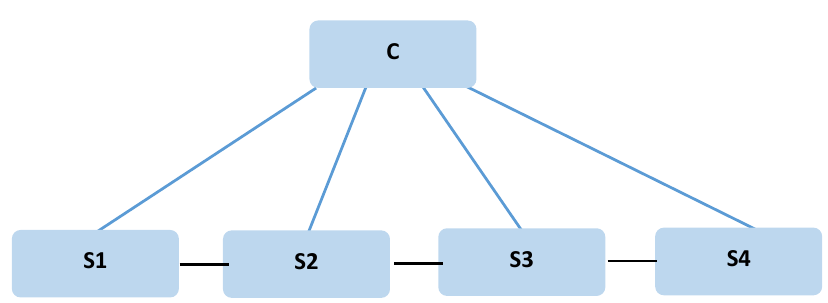
\includegraphics[scale=0.53]{images/4-1.png} \\

We call this topology, in which the four switches (S1-S4) are connected in a
single line, a linear topology. The switches are orchestrated by a single 
controller C. Your task is to rebuild this topology and simulate the 
exchange of packets over that topology in a Python simulator. Consider the
lifetime of the very first packet in the network that will be send from, for 
instance, S1 to S4: \\

The packet will be created at S1, and since it is the first packet, S1 will 
not have any flow tables installed. Instead, it will have to ask the 
controller C for a new rule. C has to install a new rule in S1. The rule 
should be: “Forward to S2”. S2 has to ask C for a new rule as  well. Note 
that in this case, the rule should be “If received from S1, forward to S3”.
Ultimately, the packet will arrive at S4, which should know that it is the 
destination of the packet. \\

Try to figure out how to build such a simulator in Python yourself first.
After that, test your system with two flows:

\begin{itemize}
\item one flow of five packets originating at S1 and with S4 as destination
\item a second flow consisting of three packets from S4 to S1
\item you do not need to acknowledge the packets in this basic simulator
\end{itemize}

\textbf{Output:} The source file $sdn\_simulator.py$ could be found under
$Exercise-4$ directory. \\
\begin{lstlisting}
$ python sdn_simulator.py                                                                                                                                                                

Welcome to SDN Simulator
NAME
         SDN SIMULATOR - an interpreter, interactive SDN simulator

OPTIONS
         <SWITCH-A> ping <SWITCH-B>
          -- Send an ICMP like request between two switches

         dump
          -- Dump all the flow tables of the switches

         exit
          -- Exit the simulator 

         help
          -- Display the help text

SDN Simulator > Enter the number of switches: 4
Creating Switches  s0...  s1...  s2...  s3...  
SDN Simulator > dump
+++++++++++++++++++
+Switch   +     s0+
+Left     +    NIL+
+Right    +    NIL+
+++++++++++++++++++
+++++++++++++++++++
+Switch   +     s1+
+Left     +    NIL+
+Right    +    NIL+
+++++++++++++++++++
+++++++++++++++++++
+Switch   +     s2+
+Left     +    NIL+
+Right    +    NIL+
+++++++++++++++++++
+++++++++++++++++++
+Switch   +     s3+
+Left     +    NIL+
+Right    +    NIL+
+++++++++++++++++++

SDN Simulator > s0 ping s3
Packet Source:  s0 Packet Desination:  s3
s0  ->  s1  ->  s2  ->  s3 (Packet delivered)

SDN Simulator > dump
+++++++++++++++++++
+Switch   +     s0+
+Left     +    NIL+
+Right    +     s1+
+++++++++++++++++++
+++++++++++++++++++
+Switch   +     s1+
+Left     +     s0+
+Right    +     s2+
+++++++++++++++++++
+++++++++++++++++++
+Switch   +     s2+
+Left     +     s1+
+Right    +     s3+
+++++++++++++++++++
+++++++++++++++++++
+Switch   +     s3+
+Left     +     s2+
+Right    +    NIL+
+++++++++++++++++++

SDN Simulator > s3 ping s0
Packet Source:  s3 Packet Desination:  s0
s3  ->  s2  ->  s1  ->  s0 (Packet delivered)

SDN Simulator > dump
+++++++++++++++++++
+Switch   +     s0+
+Left     +    NIL+
+Right    +     s1+
+++++++++++++++++++
+++++++++++++++++++
+Switch   +     s1+
+Left     +     s0+
+Right    +     s2+
+++++++++++++++++++
+++++++++++++++++++
+Switch   +     s2+
+Left     +     s1+
+Right    +     s3+
+++++++++++++++++++
+++++++++++++++++++
+Switch   +     s3+
+Left     +     s2+
+Right    +    NIL+
+++++++++++++++++++

SDN Simulator > exit
\end{lstlisting}
\end{enumerate}

%
\section{Exercise 7: MN Python API \& POX}
\subsection{The python API and Technologies (50p)}
Please explain – line by line – what happens in the following code:
\lstinputlisting[language=Python]{Exercise-7/question1.py}

\subsection{The POX controller (100P)}
One of the main features of Mininet is that you can easily port your 
emulated networks to real-world production networks. To do so, you will need 
to define a mapping of your production network to an emulated Mininet. This 
also includes the controllers you use. \\ \\
In this exercise you will have a look at the POX controller. POX is included 
in the VM image we are using for this course. What we want to do first, is 
to bring up a very simple controller implementation that acts like a 
standard hub.

\begin{itemize}
\item (Optional) You will read the solution on the next page, but think 
about  which parameters you would have to call mn with to generate a single 
switch topology with three hosts that assigns nodes with simplified MAC 
addresses, runs the Open vSwitch implementation on the switch and will link 
with an external controller. For that, we bring up a new mininet (don’t for 
get to clean up before you do  this):
\begin{lstlisting}
$ sudo mn --topo single,3 --mac --switch ovsk --controller remote
\end{lstlisting}
Now, we will bring up the POX controller in a separate terminal:
\begin{lstlisting}
$ ./pox/pox.py log.level --DEBUG misc.of_tutorial
\end{lstlisting}

\item (10P) What do you observe after connecting the controller? \\
\textbf{Solution: }  After the POX controller is enabled, the mininet 
automatically detects the presence of external controller and able to accept 
it as the controller for its setup. Hence the hosts are able to ping between 
each other. \\

We will now check if our hub is working correctly. \\

\item (20P) Open one xterm window for each host and run tcpdump on hosts 1 
and 2: \\
\textbf{Solution:} Yes, the switch acts as a hub in this case and it 
broadcasts what ever packet it receives to other devices. Hence every 
devices connected to hub receives also receives the packet received by the 
hub.

\begin{lstlisting}
$ tcpdump -XX -n -i <interface>
\end{lstlisting}

Then, in the xterm of host 3, try to ping the IP address of h1 or h2. Also 
try to ping a device that is not reachable. Please explain what you observe 
(Hint: if you recall your basic lecture on computer networks, you should 
know that a hub is generally a dumb device.)

\item (Optional) Recap how a learning switch is operating.
\item (70P) Open up the file $pox/pox/misc/of_tutorial.py$ in the editor of 
your choice. In the Python code you will see that we are currently operating 
our controller with the help of the $act_like_hub()$ method. Your task in 
this exercise is to

\begin{itemize}
\item (10P) modify the controller to use $act_like_switch()$ instead.
\item (40P) implement $act_like_switch()$ so that your controller actually
acts like a switch. There are some helpful hints in the code.
\item (20P) It is somewhat inefficient to let the controller decide the fate 
of every single packet. Implement an $act_like_flow_switch()$ method in 
which  your controller instead installs flow-rules into the switch for all 
packets that are initiually flow-table misses. This will improve the 
performance of the forwarding on subsequent packets. You can use the POX API 
and the POX documentation regarding OpenFlow here (hint: have a very close 
look at $ofp_flow_mod$).
\end{itemize}
\textbf{Solution: } Source file $of\_tutorial.py$ could be found inside 
$Exercise-7$ directory.
\end{itemize}

%
\section{Exercise 8: Mininet \& FlowVisor}
\subsection{Install FlowVisor (0P)}
(0P) To install FlowVisor, please first download it here. Now, transfer the downloaded .deb file to your VM (e.g., using scp or WinSCP), login to your VM and install the required packages for FlowVisor:
\begin{lstlisting}
$ sudo apt-get --install PATH/TO/DEB/FILE
\end{lstlisting}

\subsection{Create your own FlowVisor topology (50P)}
(50P) Using the Mininet Python API, create the FlowVisor WAN topology (which 
you may know from earlier exercises) in a file $mini-fw-topo.py$:

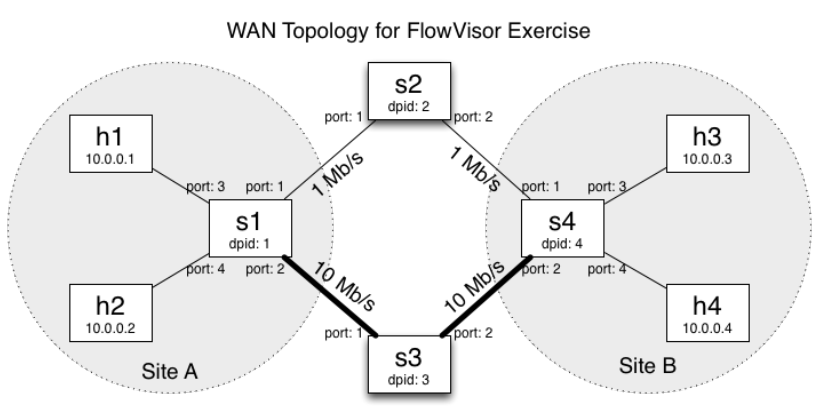
\includegraphics[scale=0.55]{images/8-1.png} 

After you have defined it start your topology
\begin{lstlisting}
$ sudo mn --custom …
\end{lstlisting}

\textbf{Solution:}
\begin{lstlisting}
$ sudo mn --custom mini-fw-topo.py --topo fvtopo --link tc
\end{lstlisting}

\subsection{Slice the Network (100p)}
Now, slice your network so that it supports the following slices:\\
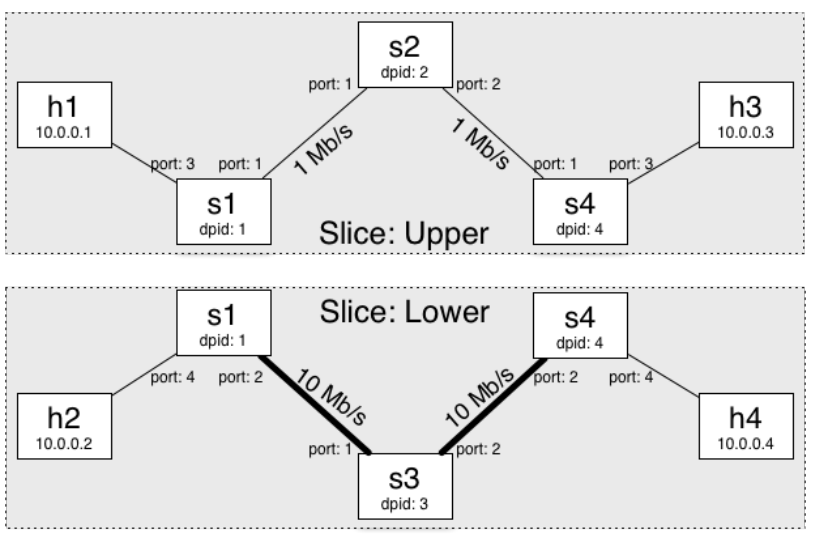
\includegraphics[scale=0.55]{images/8-2.png} 
In short, this slice arrangement allows traffic to be sent from h1 to h3 and 
h2 to h4 (and vice-versa) only, even though the topology itself (i.e., 
without slicing) would allow sending traffic between arbitrary pairs of 
hosts.\\

For slicing a network with FlowVisor in general, you need to take the 
following steps. First, make sure you set up the flowvisor package 
correctly. To configure FlowVisor, use:

\begin{lstlisting}
$ sudo -u flowvisor fvconfig generate /etc/flowvisor/config.json
\end{lstlisting}

Then, start flowvisor in a new terminal:
\begin{lstlisting}
$ sudo /etc/init.d/flowvisor start
\end{lstlisting}

We have to enable topology control for flowvisor as well:
\begin{lstlisting}
$ fvctl -f /dev/null set-config --enable-topo-ctrl
\end{lstlisting}

Similar to ovs-ofctl, fvctl is the control channel that we will use for 
flowvisor. The option –f refers to the flowvisor password file. Since we 
have set the password to be empty, we can hand it /dev/null. This part will 
be present in all the following fvctl calls. Restart flowvisor: \\

Now, have a look at FlowVisor configuration 

\begin{lstlisting}
$ fvctl -f /dev/null get-config
\end{lstlisting}

This also has the purpose of making sure that flowvisor is actually running 
and that all the switches have indeed a connection to flowvisor. The 
configuration should show this.

\begin{itemize}
\item (5P) Which part of the configuration file tells you that all four 
switches have connected to flowvisor? \\
\textbf{Solution: }
\begin{lstlisting}
"flowmod-limit": {
    "fvadmin": {
	"00:00:00:00:00:00:00:01": -1, 
	"00:00:00:00:00:00:00:02": -1, 
	"00:00:00:00:00:00:00:03": -1, 
	"00:00:00:00:00:00:00:04": -1, 
        "any": null
     }
}, 
\end{lstlisting}
In the lecture, you also got a brief overview over the major flowvisor commands. Now, make use of these commands to
\item (5P) List the currently existing slices.\\
\textbf{Solution: }
\begin{lstlisting}
mininet@mininet-vm:~$ fvctl -f /dev/null list-slices
Configured slices: fvadmin --> enabled
\end{lstlisting}

\item (5P) List the currently existing flowspaces. \\
\textbf{Solution: }
\begin{lstlisting}
mininet@mininet-vm:~$ fvctl -f /dev/null list-flowspace
Configured Flow entries:
  None
\end{lstlisting}
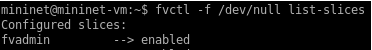
\includegraphics[scale=1]{images/8-10.png} 

\item (5P) List the currently connected switches. \\
\textbf{Solution: }
\begin{lstlisting}
mininet@mininet-vm:~$ fvctl -f /dev/null list-datapaths
Connected switches: 
	1 : 00:00:00:00:00:00:00:01
	2 : 00:00:00:00:00:00:00:02
 	3 : 00:00:00:00:00:00:00:03
 	4 : 00:00:00:00:00:00:00:04
\end{lstlisting}
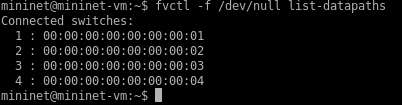
\includegraphics[scale=1]{images/8-9.png} 

\item (5P) List the currently existing links. \\
\textbf{Solution: }
\begin{lstlisting}
mininet@mininet-vm:~$ fvctl -f /dev/null list-links
[
  {
    "dstDPID": "00:00:00:00:00:00:00:02", 
    "dstPort": "1", 
    "srcDPID": "00:00:00:00:00:00:00:01", 
    "srcPort": "1"
  }, 
  {
    "dstDPID": "00:00:00:00:00:00:00:01", 
    "dstPort": "1", 
    "srcDPID": "00:00:00:00:00:00:00:02", 
    "srcPort": "1"
  }, 
  {
    "dstDPID": "00:00:00:00:00:00:00:04", 
    "dstPort": "1", 
    "srcDPID": "00:00:00:00:00:00:00:02", 
    "srcPort": "2"
  }, 
  {
    "dstDPID": "00:00:00:00:00:00:00:03", 
    "dstPort": "2", 
    "srcDPID": "00:00:00:00:00:00:00:04", 
    "srcPort": "2"
  }, 
  {
    "dstDPID": "00:00:00:00:00:00:00:01", 
    "dstPort": "2", 
    "srcDPID": "00:00:00:00:00:00:00:03", 
    "srcPort": "1"
  }, 
  {
    "dstDPID": "00:00:00:00:00:00:00:04", 
    "dstPort": "2", 
    "srcDPID": "00:00:00:00:00:00:00:03", 
    "srcPort": "2"
  }, 
  {
    "dstDPID": "00:00:00:00:00:00:00:02", 
    "dstPort": "2", 
    "srcDPID": "00:00:00:00:00:00:00:04", 
    "srcPort": "1"
  }, 
  {
    "dstDPID": "00:00:00:00:00:00:00:03", 
    "dstPort": "1", 
    "srcDPID": "00:00:00:00:00:00:00:01", 
    "srcPort": "2"
  }
]
\end{lstlisting}
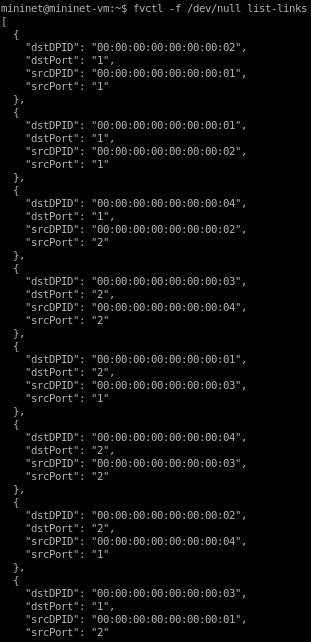
\includegraphics[scale=1]{images/8-8.png} 

Afterwards, proceed with slicing your topology:

\item (10P) Create the appropriate slices.\\
\textbf{Solution: }
\begin{lstlisting}
mininet@mininet-vm:~$ fvctl -f /dev/null add-slice upper tcp:localhost:10001 admin@upperslice
mininet@mininet-vm:~$ fvctl -f /dev/null add-slice lower tcp:localhost:10002 admin@lowerslice
mininet@mininet-vm:~$ fvctl -f /dev/null list-slices
Configured slices:
fvadmin         --> enabled 
upper           --> enabled 
lower           --> enabled
\end{lstlisting}
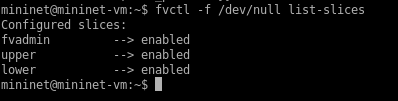
\includegraphics[scale=1]{images/8-7.png} 

\item (40P) Create the appropriate flowspaces. \\
\textbf{Solution: }
\begin{lstlisting}
mininet@mininet-vm:~$ fvctl -f /dev/null add-flowspace dpid1-port3 1 1 in_port=3 upper=7
FlowSpace dpid1-port3 was added with request id 1.
mininet@mininet-vm:~$ ^C
mininet@mininet-vm:~$ fvctl -f /dev/null add-flowspace dpid2 2 1 any upper=7
FlowSpace dpid2 was added with request id 2.
mininet@mininet-vm:~$ fvctl -f /dev/null add-flowspace dpid4-port1 4 1 in_port=1 upper=7
FlowSpace dpid4-port1 was added with request id 3.
mininet@mininet-vm:~$ fvctl -f /dev/null add-flowspace dpid4-port3 4 1 in_port=3 upper=7
FlowSpace dpid4-port3 was added with request id 4.
mininet@mininet-vm:~$ fvctl -f /dev/null add-flowspace dpid1-port2 1 1 in_port=2 lower=7
FlowSpace dpid1-port2 was added with request id 5.
mininet@mininet-vm:~$ fvctl -f /dev/null add-flowspace dpid1-port4 1 1 in_port=4 lower=7
FlowSpace dpid1-port4 was added with request id 6.
mininet@mininet-vm:~$ fvctl -f /dev/null add-flowspace dpid3 3 1 any lower=7
FlowSpace dpid3 was added with request id 7.
mininet@mininet-vm:~$ fvctl -f /dev/null add-flowspace dpid4-port2 4 1 in_port=2 lower=7
FlowSpace dpid4-port2 was added with request id 8.
mininet@mininet-vm:~$ fvctl -f /dev/null add-flowspace dpid4-port4 4 1 in_port=4 lower=7
FlowSpace dpid4-port4 was added with request id 9.
mininet@mininet-vm:~$ fvctl -f /dev/null add-flowspace dpid1-port1 1 1 in_port=1 upper=7
FlowSpace dpid1-port1 was added with request id 10.
\end{lstlisting}

\begin{lstlisting}
mininet@mininet-vm:~$ fvctl -f /dev/null list-flowspace
Configured Flow entries:
{"force-enqueue": -1, "name": "dpid1-port1", "slice-action": [{"slice-name": "upper", "permission": 7}], "queues": [], "priority": 1, "dpid": "00:00:00:00:00:00:00:01", "id": 1, "match": {"wildcards": 4194302, "in_port": 1}}
{"force-enqueue": -1, "name": "dpid1-port3", "slice-action": [{"slice-name": "upper", "permission": 7}], "queues": [], "priority": 1, "dpid": "00:00:00:00:00:00:00:01", "id": 2, "match": {"wildcards": 4194302, "in_port": 3}}
{"force-enqueue": -1, "name": "dpid2", "slice-action": [{"slice-name": "upper", "permission": 7}], "queues": [], "priority": 1, "dpid": "00:00:00:00:00:00:00:02", "id": 3, "match": {"wildcards": 4194303}}
{"force-enqueue": -1, "name": "dpid4-port1", "slice-action": [{"slice-name": "upper", "permission": 7}], "queues": [], "priority": 1, "dpid": "00:00:00:00:00:00:00:04", "id": 4, "match": {"wildcards": 4194302, "in_port": 1}}
{"force-enqueue": -1, "name": "dpid4-port3", "slice-action": [{"slice-name": "upper", "permission": 7}], "queues": [], "priority": 1, "dpid": "00:00:00:00:00:00:00:04", "id": 5, "match": {"wildcards": 4194302, "in_port": 3}}
{"force-enqueue": -1, "name": "dpid1-port2", "slice-action": [{"slice-name": "lower", "permission": 7}], "queues": [], "priority": 1, "dpid": "00:00:00:00:00:00:00:01", "id": 6, "match": {"wildcards": 4194302, "in_port": 2}}
{"force-enqueue": -1, "name": "dpid1-port4", "slice-action": [{"slice-name": "lower", "permission": 7}], "queues": [], "priority": 1, "dpid": "00:00:00:00:00:00:00:01", "id": 7, "match": {"wildcards": 4194302, "in_port": 4}}
{"force-enqueue": -1, "name": "dpid3", "slice-action": [{"slice-name": "lower", "permission": 7}], "queues": [], "priority": 1, "dpid": "00:00:00:00:00:00:00:03", "id": 8, "match": {"wildcards": 4194303}}
{"force-enqueue": -1, "name": "dpid4-port2", "slice-action": [{"slice-name": "lower", "permission": 7}], "queues": [], "priority": 1, "dpid": "00:00:00:00:00:00:00:04", "id": 9, "match": {"wildcards": 4194302, "in_port": 2}}
{"force-enqueue": -1, "name": "dpid4-port4", "slice-action": [{"slice-name": "lower", "permission": 7}], "queues": [], "priority": 1, "dpid": "00:00:00:00:00:00:00:04", "id": 10, "match": {"wildcards": 4194302, "in_port": 4}}
{"force-enqueue": -1, "name": "dpid1-port1", "slice-action": [{"slice-name": "upper", "permission": 7}], "queues": [], "priority": 1, "dpid": "00:00:00:00:00:00:00:01", "id": 11, "match": {"wildcards": 4194302, "in_port": 1}}
\end{lstlisting}
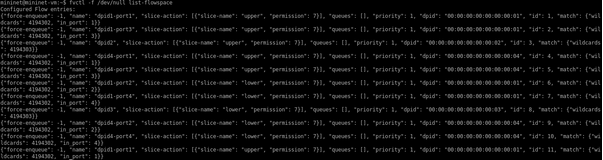
\includegraphics[scale=0.745]{images/8-6.png} 

\item (10P) Connect an instance of the POX controller to each of your slices 
\\
\textbf{Solution: }\\
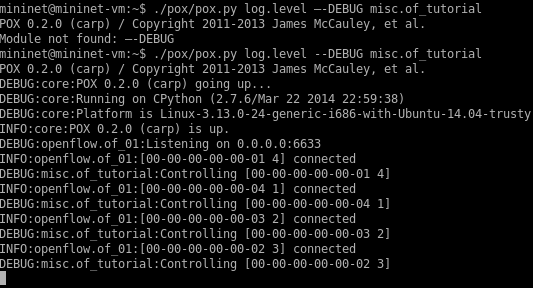
\includegraphics[scale=0.815]{images/8-3.png} 
\item (10P) In Mininet, verify that your slicing works properly, i.e., h1 
can reach h3 but not h2 and h4, and h2 can reach h4, but not h1 and h3. \\
\textbf{Solution: } \\
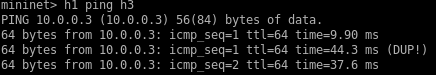
\includegraphics[scale=1]{images/8-4.png}  \\
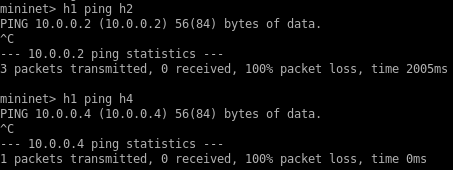
\includegraphics[scale=.9625]{images/8-5.png} 
\end{itemize}

%
\section{Paper Review}
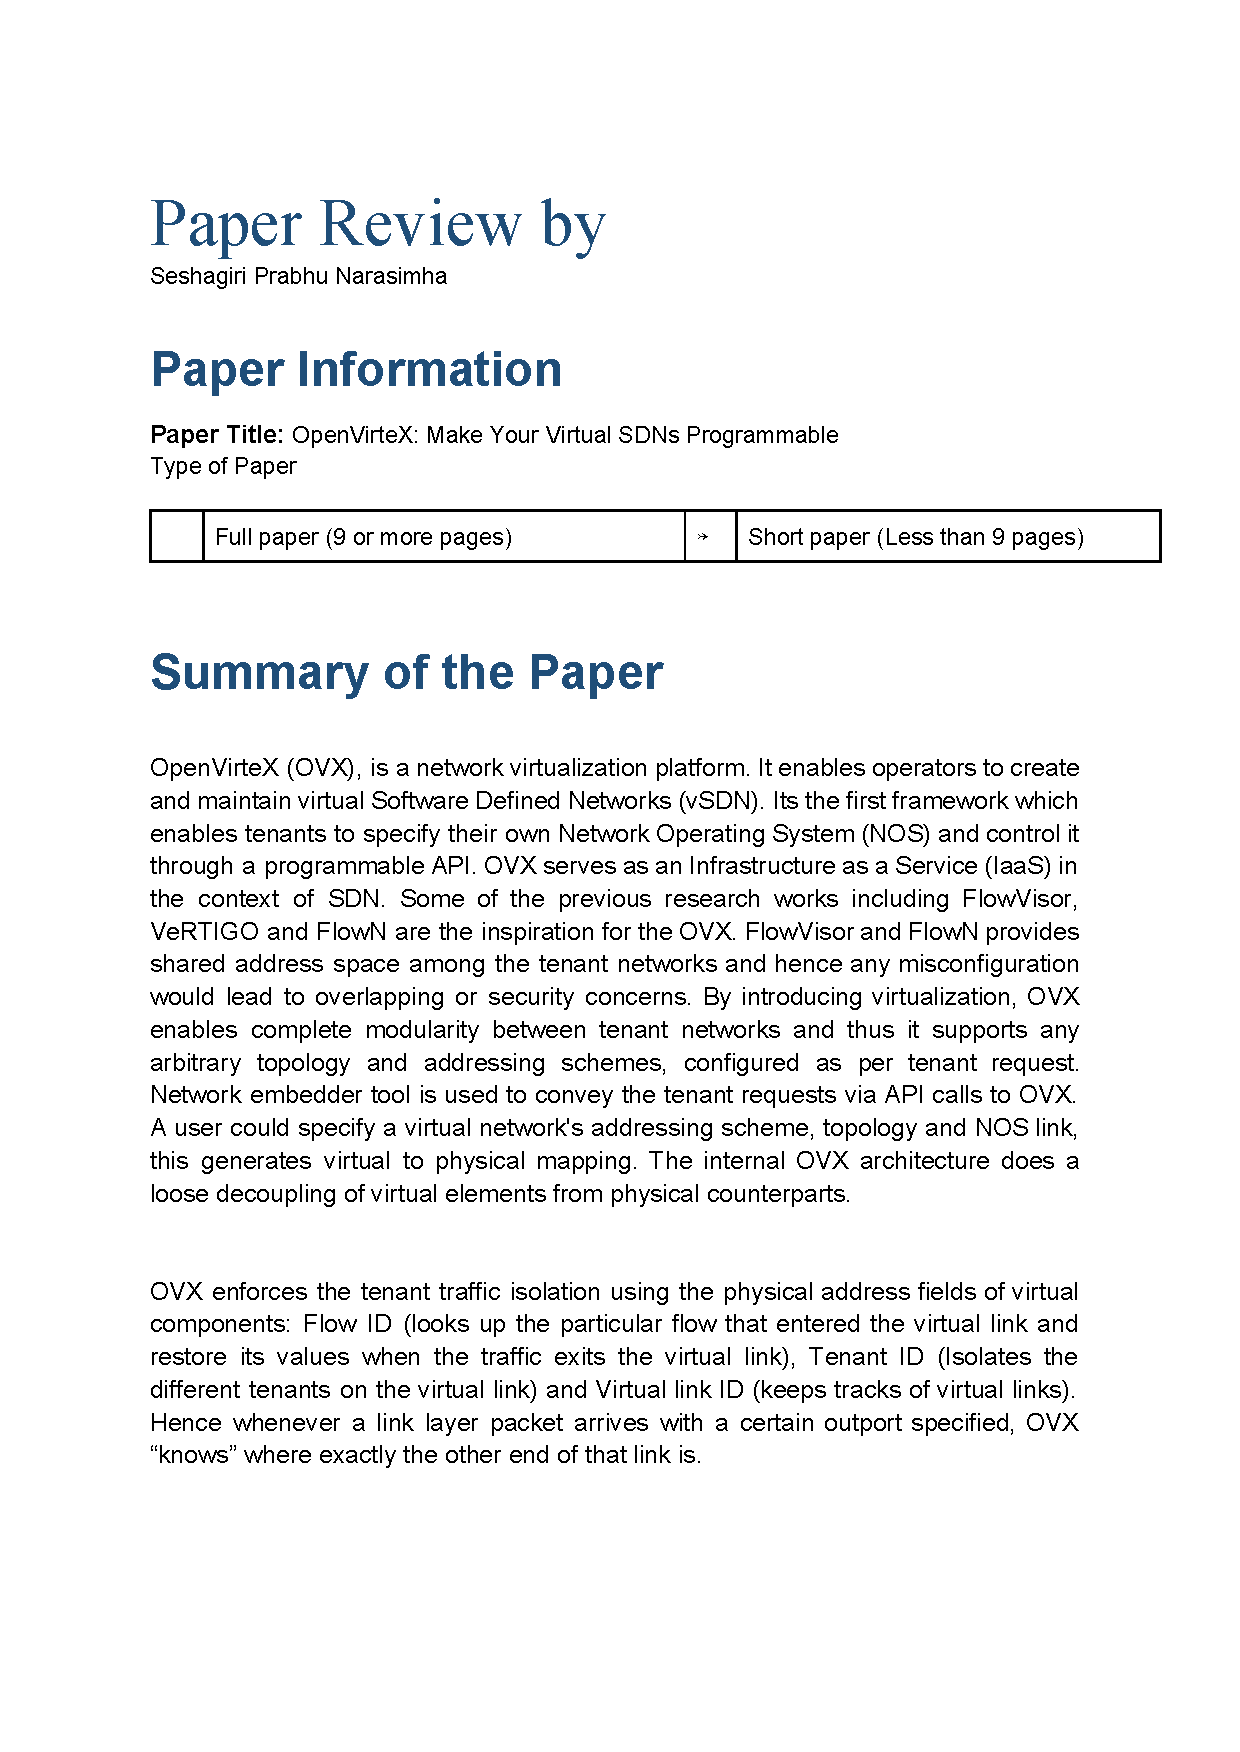
\includepdf[pages=-]{documents/PaperReview.pdf}

%
\section{Presentation}
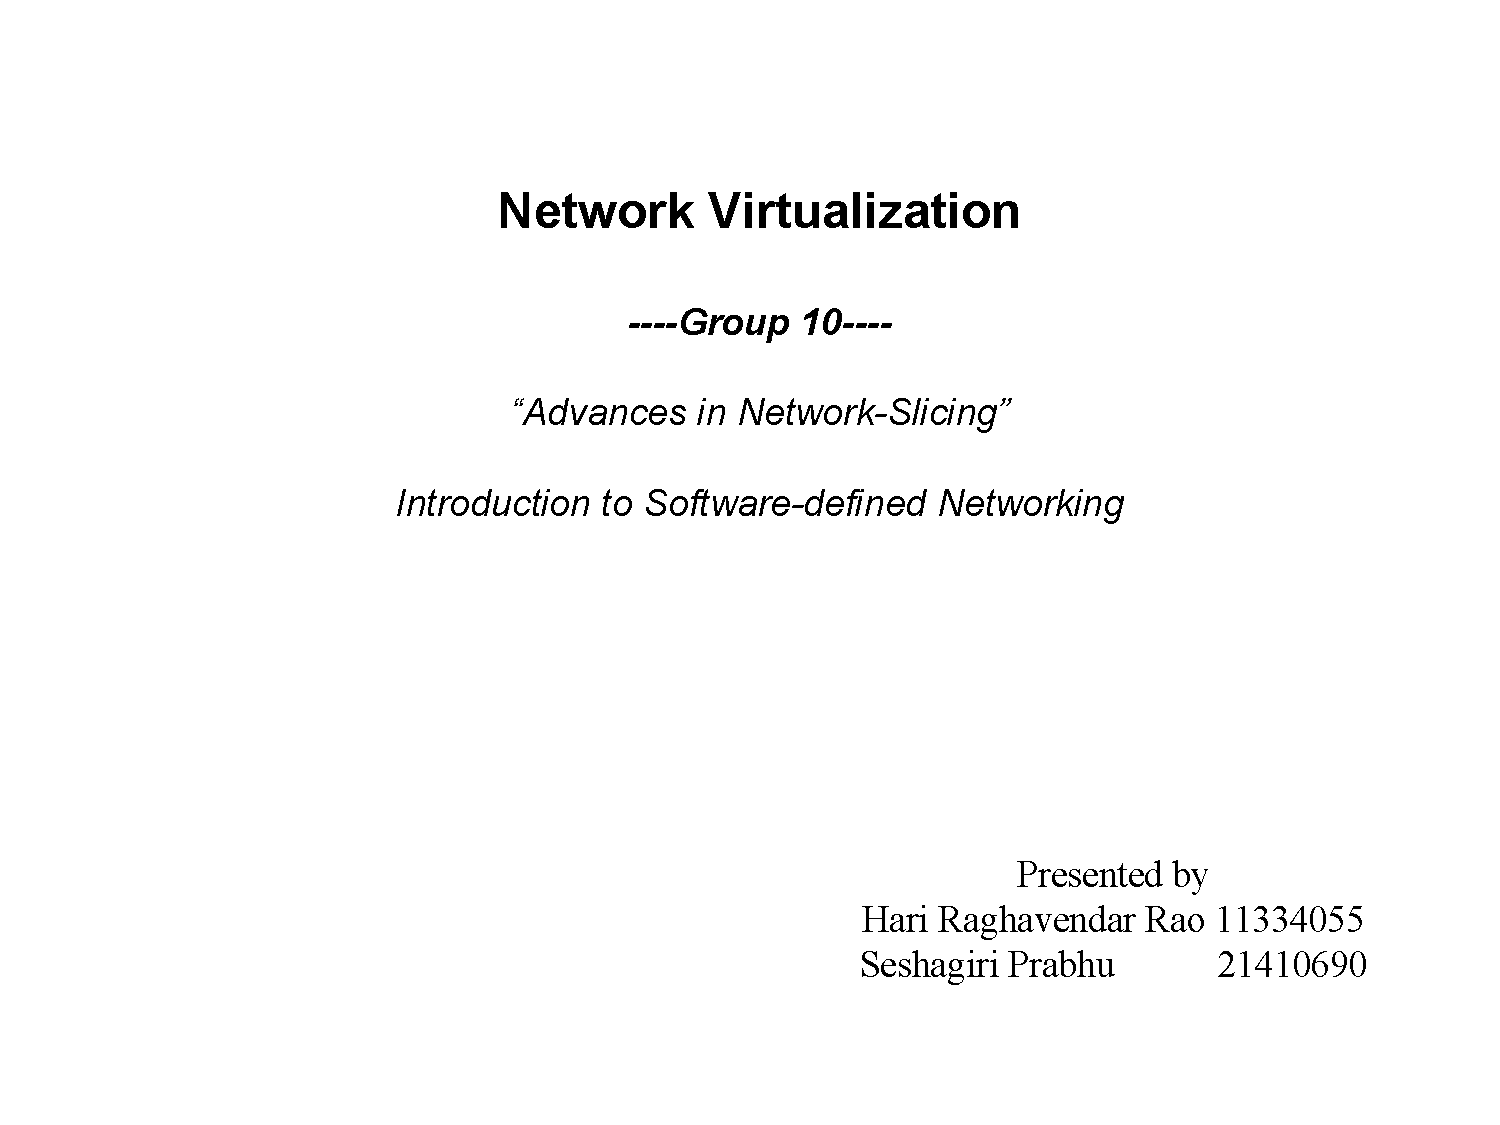
\includepdf[pages=-]{documents/presentation.pdf}
\end{document}
